%===================================================================================
% Chapter: Annotation model
%===================================================================================
\Chapter{Modelo de Anotación}\label{chapter:annotation_model}
El primer paso para el algoritmo presentado en este trabajo, es tener un corpus\footnote{Un corpus es un conjunto de oraciones y/o documentos de ejemplos reales usados en el lenguaje natural.} anotado basado en el esquema presentado a continuación. Además, en este capítulo son analizadas algunas estadísticas de un corpus de oraciones del dominio médico en idioma español. Esto es utilizado en la presente investigación. También son mostradas las herramientas empleadas para construirlo y trabajar con el mismo.
%===================================================================================

\section{Esquema de anotación}
\label{section:annotation_structure}
El modelo de anotación de propósito general empleado busca capturar los rasgos y relaciones semánticas más relevantes presentes en oraciones del lenguaje natural. Este debe evitar ambigüedades tanto como sea posible, de forma que anotadores humanos distintos tengan una alta probabilidad de coincidir. A la misma vez, necesita ser lo suficientemente expresivo para representar los conceptos relevantes del dominio y sus interacciones. Además, debe ser capaz de construir conceptos complejos a partir de combinar otros más simples mediante el uso de un conjunto reducido de reglas. También está diseñado para asistir en desarrollo de sistemas de descubrimiento de conocimiento. Por este motivo es necesario independizar la representación del modelo de la estructura gramatical de las oraciones, y en su lugar, tratar de representar el significado semántico.

Este modelo de anotación se basa en las tripletas \textit{Subject-Action-Target} (en español \textit{Sujeto-Acción-Objetivo}) y en la estructura gramatical \textit{sujeto-verbo-objeto}, normalmente expresada con su abreviatura \textbf{SVO}. Tiende a ser el orden predeterminado porque el verbo se usa para dividir el sujeto del predicado, sin necesidad de usar partículas para indicar dónde empiezan o terminan los mismos. Además, es una de las secuencias más frecuente en el lenguaje natural y de hecho es usada en la mayoría de lenguas occidentales y un buen número de orientales~\cite{ref:83}.

\begin{figure}[H]
	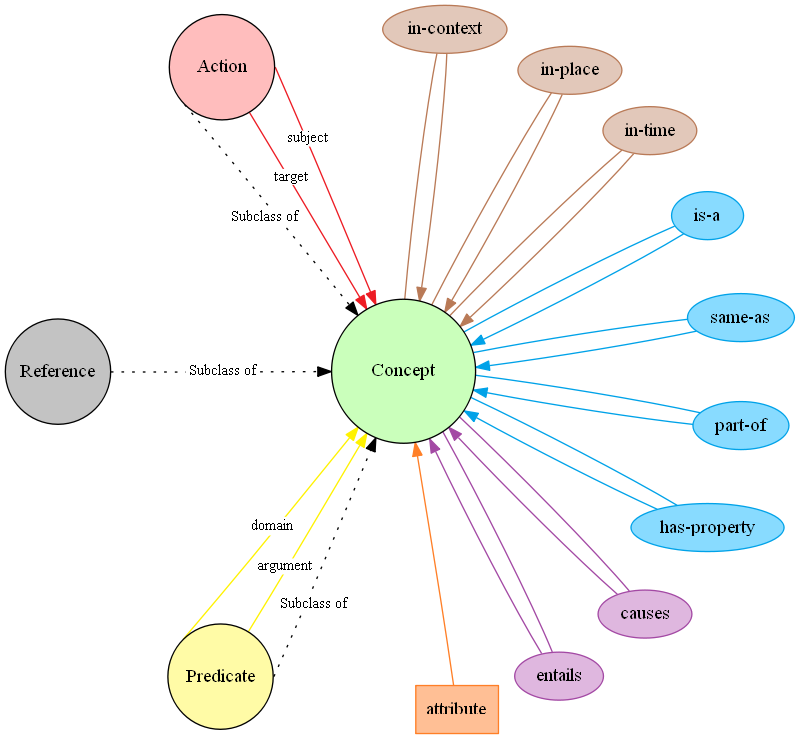
\includegraphics[width=\linewidth]{graphics/annotation_model.png}
	\caption[Esquema conceptual del modelo de anotación]{Esquema conceptual del modelo de anotación.}
	\label{fig:annotation_model}
\end{figure}

Es válido destacar que al estar interesados en fragmentos de conocimiento, el rol semántico de las entidades anotadas puede no coincidir con su rol gramatical. Los roles semánticos fundamentales de este modelo son \textit{Concept} y \textit{Action} (en español \textit{Concepto} y \textit{Acción} respectivamente), siendo usados para representar información objetiva acerca de lo que se está haciendo, por quién, y a quién. Estas estructuras pueden ser contextualizadas en tiempo, lugar y otras circunstancias generales.

Existen otros 2 roles semánticos, llamados \textit{Predicate} y \textit{Reference} (en español \textit{Predicado} y \textit{Referencia} respectivamente). \textit{Predicate} es utilizado para construir conceptos más complejos a partir de otros más simples. \textit{Reference} define un término del que se menciona un hecho, pero en el contexto de la oración no está escrito explícitamente, por lo que la información semántica de este rol no está contenida en las anotaciones.

Por último, son usadas seis relaciones con semántica específica para representar conocimiento de propósito general. Las relaciones
\textit{is-a}, \textit{part-of}, \textit{same-as} y \textit{has-property} (en español \textit{es-un}, \textit{parte-de}, \textit{igual-que} y \textit{tiene-propiedad} respectivamente) son tomadas de representaciones ontológicas y taxonómicas, mientras que \textit{causes} y \textit{entails} (en español \textit{causa} e \textit{implica} respectivamente) se toman del dominio de la comprensión del texto. Además, las relaciones \textit{in-time}, \textit{in-place} e \textit{in-context} (en español \textit{en-tiempo}, \textit{en-lugar} y \textit{en-contexto} respectivamente) son usadas para dar contexto y cuatro atributos booleanos son asociados a los conceptos. Las próximas secciones explican cada rol semántico y las relaciones detalladamente, incluyendo ejemplos de su uso en oraciones del lenguaje natural.

La figura \ref{fig:annotation_model} muestra una representación gráfica del modelo de anotación. En el esquema conceptual se puede apreciar que cada uno de los roles semánticos definidos en el modelo de anotación está representado por un círculo. Además, las posibles relaciones definidas entre cada pareja de roles se representan con óvalos y con un rectángulo los atributos que pueden tener los mismos. En color café están representadas las relaciones de contexto, en azul las taxonómicas y en violeta las de causalidad e implicación.

\subsection{Conceptos}
El rol \textit{Concept} es usado para anotar fragmentos de texto que representan una unidad atómica de información en el dominio. Puede ser una entidad nombrada, un sustantivo, adjetivo o verbo, que representa un concepto relevante en el dominio del texto. Por ende, la gran mayoría de palabras o frases que expresan un significado propio es anotado de esta manera (o uno de sus derivados, como se explica más adelante). Palabras tales como artículos, preposiciones y conjunciones, las cuales solo realizan una función gramatical y sin significado semántico, no son anotados.

\begin{figure}[H]
	\begin{center}
		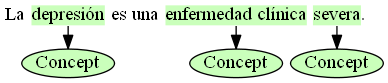
\includegraphics[width=3.5in]{graphics/annotation_example_concept.png}
		\caption[Anotación de conceptos]{Ejemplo de anotación de conceptos.}
		\label{fig:annotation_example_concept}
	\end{center}
\end{figure}

\vspace{-0.8cm}
En la figura \ref{fig:annotation_example_concept} se distinguen claramente como conceptos en el dominio médico las palabras \guillemot{\texttt{depresión}} y \guillemot{\texttt{severa}}, cuyo significado de cada uno de ellos es independiente del rol gramatical que tengan en la oración. Algunos conceptos, como \guillemot{\texttt{enfermedad clínica}} en este caso, se componen de múltiples palabras, ya sea porque de manera independiente no tienen relevancia, o porque al unirlos cobra un significado diferente al de sus componentes individuales. En esta ocasión, a pesar de que \guillemot{\texttt{enfermedad}} y \guillemot{\texttt{clínica}} poseen una connotación bien definida por sí mismas, el concepto \guillemot{\texttt{enfermedad clínica}} tiene gran importancia en el dominio médico, lo cual lo hace una unidad única de información, es decir, un especialista en este campo puede identificarla claramente. Las palabras que conforman un concepto no tienen que estar consecutivas en el texto, pero sí son seleccionadas de izquierda a derecha.

\subsection{Acciones}
El rol \textit{Action} es un tipo particular de \textit{Concept} que indica una acción o evento que otro concepto puede realizar o ser objetivo de ella. Un \textit{Action} puede ser enlazado con otros conceptos relevantes a partir de 2 roles semánticos: \textit{subject} y \textit{target} (en español \textit{sujeto} y \textit{objetivo} respectivamente). El \textit{subject} es el que produce la acción, mientras que el \textit{target} es el que recibe los efectos o el objetivo de la acción.

En la figura \ref{fig:annotation_example_action} la acción es indicada por una palabra con el rol gramatical de verbo. Intuitivamente este es el caso más común, sin embargo, una acción puede ser indicada además por una palabra con otro rol gramatical, como los sustantivos. Por ejemplo, en la frase \doublequote{\textit{\dots\space el empeoramiento de los síntomas \dots}}, la palabra \guillemot{\texttt{empeoramiento}} se considera también un \textit{Action} a pesar de que no es un verbo, dado que describe un proceso o evento que ocurre sobre otros conceptos.

Por tanto, el rol semántico \textit{Action} describe el significado de un concepto en el dominio semántico, en lugar de su función gramatical en una oración específica. Si un concepto del dominio expresa un proceso o evento que realiza otro concepto o produce un efecto sobre otro(s), entonces es un \textit{Action}, incluso si puede ser usado con una función gramatical distinta.

\begin{figure}[H]
	\begin{center}
		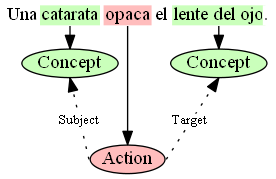
\includegraphics[height=1.7in]{graphics/annotation_example_action.png}
		\caption[Anotación de acción]{Ejemplo de anotación de acción.}
		\label{fig:annotation_example_action}
	\end{center}
\end{figure}

\vspace{-0.4in}
\subsection{Referencias}
El rol \textit{Reference} es un tipo de \textit{Concept} que no tiene un significado semántico específico, pero que es necesario por razones gramaticales. Es usado para anotar pronombres (por ejemplo, \textit{este}, \textit{aquel}) y demás elementos que hacen referencia a otro \textit{Concept} presente en la oración, documento y/o corpus. En la figura \ref{fig:annotation_example_reference_and_predicate} puede verse un ejemplo.

\begin{figure}[H]
	\begin{center}
		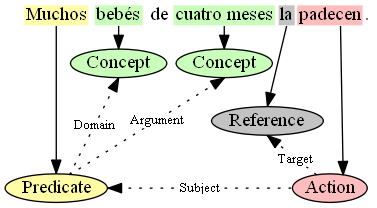
\includegraphics[width=3.4in]{graphics/annotation_example_reference_and_predicate.png}
		\caption[Anotación de referencia y predicado]{Ejemplo de anotación de referencia y predicado.}
		\label{fig:annotation_example_reference_and_predicate}
	\end{center}
\end{figure}


\subsection{Predicados}
El rol \textit{Predicate} es usado para formar conceptos más complejos a partir de aplicar un determinado criterio sobre otros en una oración. Un caso de uso común es para definir el subconjunto perteneciente a un concepto y que cumple determinadas propiedades.

Por ejemplo, en la figura \ref{fig:annotation_example_reference_and_predicate}, la palabra \textit{muchos} cumple la función de filtrar algunos de los bebés, por eso es anotada como \textit{Predicate}.

De conjunto con esta relación, cualquier concepto puede jugar dos roles adicionales: \textit{domain} y \textit{argument} (en español \textit{dominio} y \textit{argumento} respectivamente), completando así su significado. El \textit{Predicate} define el conjunto de objetos pertenecientes al dominio (el concepto enlazado con el rol \textit{domain}) que cumplen el predicado anotado según los argumentos señalados (el o los conceptos anotados con el rol \textit{argument}).

De forma matemática, la relación \textit{Predicate} define al conjunto:

\begin{center}
	$\{x\in Domain~|~Predicate(x,~arg_1,~arg_2,\dots,~arg_n)\}$
\end{center}

En el ejemplo de la figura \ref{fig:annotation_example_reference_and_predicate}, el dominio de este \textit{Predicate} es representado por el \textit{Concept} \guillemot{\texttt{bebés}}, y el único argumento es \guillemot{\texttt{cuatro meses}}. Esta construcción da lugar a un nuevo concepto, el de \guillemot{\texttt{muchos bebés de 4 meses}}, el cual puede ser entendido como la aplicación del filtro \guillemot{\texttt{muchos}} sobre el conjunto de elementos definido por el \textit{Concept} \guillemot{\texttt{bebés}}, de los cuales son seleccionados aquellos con el argumento \guillemot{\texttt{cuatro meses}}.

\begin{center}
	$\{x\in Beb\acute{e}s~|~muchos(x,~cuatro~meses)\}$
\end{center}

El nuevo concepto complejo construido de esta forma es representado
en la oración por la anotación \textit{Predicate} en sí misma. Por tanto, para continuar con el ejemplo anterior, en caso de querer que estos \guillemot{\texttt{muchos bebés}} jugaran el rol \textit{subject} o \textit{target}, la anotación correspondiente debe ir desde un \textit{Action} hacia el \textit{Predicate}, como se muestra en la figura \ref{fig:annotation_example_reference_and_predicate}. Es un error anotar que el \textit{subject} de \guillemot{\texttt{padecen}} es \guillemot{\texttt{bebés}} porque este concepto representa \guillemot{\texttt{todos los bebés}}. Por ende, el \textit{Predicate} es usado para representar el concepto filtrado en sí, no el operador de filtrado.

Como caso de uso particular de esta anotación, se encuentra el caso en que un término no representa un concepto relevante por sí mismo (por tanto no debe ser anotado como \textit{Concept}), sino que denota una propiedad o rasgo medible de otro concepto. Por ejemplo, \guillemot{\texttt{tipo}}, \guillemot{\texttt{parte}}, \guillemot{\texttt{nivel}} y \guillemot{\texttt{cada}} en \doublequote{\textit{tipo de cáncer}}, \doublequote{\textit{parte del cuerpo}}, \doublequote{\textit{nivel de glucosa}} y \doublequote{\textit{cada trimestre}} respectivamente.
En tales casos, el \textit{Predicate} debe carecer de alguno de los roles \textit{domain} o \textit{argument}. Si el tipo o clase resultante de formar el predicado coincide con el del concepto a enlazar, entonces el rol utilizado es \textit{domain}. En otro caso, se enlaza al concepto con el rol \textit{argument}.

\subsection{Componiendo conceptos}
\label{section:composing_concepts}
Así como un \textit{Predicate} puede utilizarse para componer conceptos, se puede lograr un resultado similar al considerar un \textit{Action} como el \textit{subject} o \textit{target} de otro.

\begin{figure}[H]
	\begin{center}
		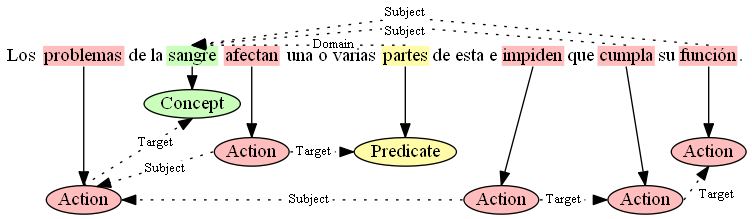
\includegraphics[width=\textwidth]{graphics/annotation_example_composing_concepts.png}
		\caption[Anotación de conceptos compuestos]{Ejemplo de anotación de conceptos compuestos.}
		\label{fig:annotation_example_composing_concepts}
	\end{center}
\end{figure}

Por ejemplo, en la figura \ref{fig:annotation_example_composing_concepts}, hay un concepto complejo formado con las palabras \guillemot{\texttt{problemas}} y \guillemot{\texttt{sangre}}. Este a su vez, actúa como \textit{subject} de \guillemot{\texttt{afectan}}, dado que no todos los \guillemot{\texttt{problemas}} se \guillemot{\texttt{afectan}}, sino solo aquellos que son \guillemot{\texttt{problemas de la sangre}}. Por otro lado, la propia palabra \guillemot{\texttt{sangre}} actúa como \textit{domain} del predicado \guillemot{\texttt{partes}}, el cual es el \textit{target} de \guillemot{\texttt{afectan}}. De manera similar sucede con los otros tres conceptos complejos \guillemot{\texttt{impiden}}, \guillemot{{cumpla}} y \guillemot{\texttt{función}}.

De esta forma puede apreciarse que la construcción y/o anotación de conceptos complejos es una tarea compleja en sí. Además, esta estrategia puede ser usada para representar la nominalización de un verbo, pues al anotar el \textit{Action} y los correspondientes \textit{subject} y \textit{target} se
construye el concepto complejo.

\subsection{Relaciones taxonómicas}
Los roles \textit{Action} y \textit{Concept} permiten capturar gran parte del significado semántico de una oración a partir de anotar como acción todos los conceptos que indican alguna interacción entre ellos. Sin embargo, algunos tipos específicos de interacciones son tan comunes que son considerados en diferentes dominios del conocimiento como los bloques constructores para las representaciones ontológicas y taxonómicas. Tal es el caso de las parejas de hiperonimia/hiponimia, anotadas como relaciones \textit{is-a} (en español \textit{es-un}) y meronimia/holonimia, anotadas como relaciones \textit{part-of} (en español \textit{parte-de}), que forman el centro de muchas bases de conocimiento.

Estos dos tipos de relaciones son muy comunes en la mayoría de los dominios del conocimiento, y hay muchas formas distintas para expresar estas ideas en texto. Debido a ello, resulta mejor representarlas explícitamente como relaciones entre conceptos, en lugar de recurrir a anotar como \textit{Action} las formas del verbo ser o estar. Además, una anotación explícita de estas relaciones permite que sistemas de descubrimiento de conocimiento entrenados en estas anotaciones extraigan estructuras más compactas y concisas, dado que no es necesario realizar interpretaciones adicionales.

Las relaciones \textit{is-a} y \textit{part-of} pueden ser indicadas explícitamente en el texto por la aparición de patrones textuales comunes, como es el caso de los patrones de Hearst~\cite{ref:14}. Sin embargo, aun cuando no ocurrieran en el texto indicaciones explícitas de estas relaciones, se considera su anotación.

En la figura \ref{fig:annotation_example_is_a} puede verse un ejemplo de anotación de la relación \textit{is-a}. En esta oración, las palabras \guillemot{\texttt{hepatitis}} e \guillemot{\texttt{hígado}} son claramente conceptos, mientras que \guillemot{\texttt{inflamación}} es una acción. Como se ha visto anteriormente, una relación con un rol complejo, es decir, un rol que esté relacionado hacia otros roles, implica la relación con él como un todo y no solo con su significado semántico. Por ende, \guillemot{\texttt{hepatitis} \textit{is-a} \texttt{inflamación del hígado}} es el resultado de la anotación de esta oración.

Por otra parte, en la figura \ref{fig:annotation_example_part_of} se puede apreciar un ejemplo de la relación \textit{part-of}. En esta oración son anotadas como conceptos la palabra \guillemot{\texttt{depresión}} y la frase \guillemot{\texttt{trastorno bipolar}}. Esta oración, a modo de anotación, resulta en \guillemot{\texttt{depresión} \textit{part-of} \texttt{trastorno bipolar}}.

Las parejas de sinonimia, anotadas como relaciones \textit{same-as} (en español \textit{igual-que}) es usada para indicar sinónimos o conceptos que son considerados iguales en el dominio del documento. Puede ser usada cuando un concepto simple es definido a partir de describirlo como otro concepto más complejo.

\begin{figure}[H]
	\centering
	\begin{subfigure}{3.1in}
		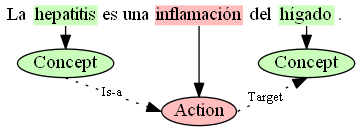
\includegraphics[width=\textwidth]{graphics/annotation_example_is_a.png}
		\caption{Ejemplo de anotación de hiperonimia e hiponimia.}
		\vspace{0.4in}
		\label{fig:annotation_example_is_a}
	\end{subfigure}
	\begin{subfigure}{3.25in}
		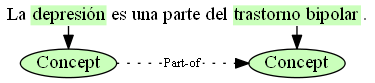
\includegraphics[width=\linewidth]{graphics/annotation_example_part_of.png}
		\caption{Ejemplo de anotación de meronimia y holonimia.}
		\vspace{0.4in}
		\label{fig:annotation_example_part_of}
	\end{subfigure}
	\begin{subfigure}{4.2in}
		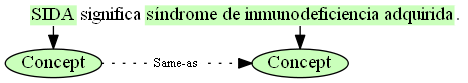
\includegraphics[width=\linewidth]{graphics/annotation_example_same_as.png}
		\caption{Ejemplo de anotación de sinonimia.}
		\vspace{0.4in}
		\label{fig:annotation_example_same_as}
	\end{subfigure}
	\begin{subfigure}{3.9in}
		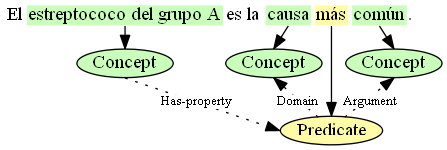
\includegraphics[width=\linewidth]{graphics/annotation_example_has_property.png}
		\caption{Ejemplo de anotación de propiedad.}
		\label{fig:annotation_example_has_property}
	\end{subfigure}
	\caption{Anotación de las relaciones taxonómicas}
\end{figure}

La figura \ref{fig:annotation_example_same_as} muestra un ejemplo de anotación de la relación \textit{same-as}. La palabra \guillemot{\texttt{SIDA}} y la frase \guillemot{\texttt{síndrome de inmunodeficiencia adquirida}} son anotadas como conceptos. Por tanto, esta oración a modo de anotación queda \guillemot{\texttt{SIDA} \textit{same-as} \texttt{síndrome de inmunodeficiencia adquirida}}.

Las propiedades, anotadas como relaciones \textit{has-property} (traducido al español como \textit{tiene-propiedad}) es usada para especificar que un concepto tiene una propiedad, característica, o puede ser descrita por otro concepto. Sin embargo, este tipo de relación puede conllevar a ciertas dificultades, como por ejemplo la paradoja de Bertrand Russell~\cite{ref:15} y la de Grelling-Nelson~\cite{ref:16}. Además, una propiedad puede implicar gran cantidad de propiedades e incluso una cantidad infinita de ellas. Por ejemplo si \guillemot{\texttt{la persona pesa más de 60 kilogramos}} entonces también se cumple que \guillemot{\texttt{la persona pesa más de 59 kilogramos}} y por consiguiente, que \guillemot{\texttt{la persona pesa más de 58 kilogramos}}. De manera similar, dado que en este caso, el peso es un valor numérico decimal, se pueden construir infinitas propiedas de este tipo. Esto cobra especial importancia a la hora de crear e interpretar la base de conocimientos explicada en el capítulo \ref{chapter:proposed_solution}. Puesto que no pueden crearse infinitas relaciones, y por tanto, la interpretación de estas es dependiente del contexto en que se esté analizando.

En la figura \ref{fig:annotation_example_has_property} se puede observar un ejemplo de la anotación \textit{has-property}. En esta oración son anotadas la frase \guillemot{\texttt{estreptococo del grupo A}} y las palabras \guillemot{\texttt{causa}} y \guillemot{\texttt{común}} como conceptos. También, la palabra \guillemot{\texttt{más}} es anotada como un predicado, en conjunto con \guillemot{\texttt{causa}} y \guillemot{\texttt{común}} como dominio y argumento respectivamente. Al ser anotada la relación \textit{has-property}, la anotación resulta como \guillemot{\texttt{estreptococo del grupo A} \textit{has-property} \texttt{causa más común}}.

Para todas las relaciones taxonómicas, solo se considera su anotación cuando la oración implica la existencia de ella, aun cuando fuese implícita. En ningún caso se anota basada solamente en conocimiento externo o del dominio.

\vspace{-0.2in}
\subsection{Causalidad e implicación}
Las cuatro relaciones semánticas presentadas hasta ahora son útiles para capturar la estructura taxonómica del conocimiento expresado en textos del lenguaje natural. Dos relaciones adicionales son definidas para construir conexiones lógicas entre conceptos: \textit{causes} y \textit{entails} (en español \textit{causa} e \textit{implica} respectivamente). La relación \textit{causes} es usada para expresar que un evento, identificado en general como un concepto, es una posible causa para otro evento. En la figura \ref{fig:annotation_example_causes} se muestra un ejemplo anotado.

Esta relación indica causalidad, no correlación ni implicación lógica. Por tanto, debe estar declarado con claridad en la oración que hay una conexión de causa directa entre ambos eventos. Además, hay un grado de incertidumbre implicada en la causalidad, lo cual significa que si \guillemot{\texttt{A} \textit{causes} \texttt{B}}, eso no necesariamente implica que cada vez que pase \guillemot{\texttt{A}} sería seguido por \guillemot{\texttt{B}}, ni que en cualquier caso que ocurra \guillemot{\texttt{B}} será a causa de \guillemot{\texttt{A}}.

En contraste, la relación \textit{entails} es usada para denotar implicación lógica. En este caso, no es necesario que los eventos estén relacionados por causalidad; lo único que debe cumplirse es que cuando la proposición \guillemot{\texttt{A}} es verdadera entonces siempre sucede el caso de que la proposición \guillemot{\texttt{B}} es verdadera. En la figura \ref{fig:annotation_example_entails} puede verse un ejemplo, donde un concepto complejo, en este caso \guillemot{\texttt{tener}} implica \guillemot{\texttt{necesita}}, el cual es también un concepto complejo. Desde otro punto de vista, la anotación de esa oración resulta en:

\vspace{-0.05in}
\begin{center}
	\guillemot{$\big($tener [suficiente energía] en el cuerpo$\big)$\\\textit{entails}\\(necesitar glucosa en el cuerpo)}
\end{center}

\vspace{-0.05in}
\begin{figure}[H]
	\centering
	\begin{subfigure}{3.25in}
		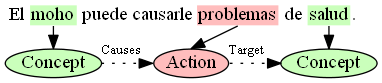
\includegraphics[width=\textwidth]{graphics/annotation_example_causes.png}
		\caption{Ejemplo de anotación de causalidad.}
		\vspace{0.4in}
		\label{fig:annotation_example_causes}
	\end{subfigure}
	\begin{subfigure}{3.9in}
		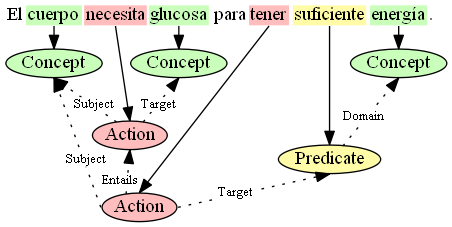
\includegraphics[width=\linewidth]{graphics/annotation_example_entails.png}
		\caption{Ejemplo de anotación de implicación.}
		\label{fig:annotation_example_entails}
	\end{subfigure}
	\caption{Anotación de causalidad e implicación}
\end{figure}

\vspace{-0.1in}
La anotación de causalidad e implicación evita anotar varias palabras y frases que comparten el mismo significado semántico. Por ejemplo, en la figura \ref{fig:annotation_example_causes} no resulta necesario anotar \guillemot{\texttt{puede causarle}} debido a que el significado correcto está siendo representado por la relación \textit{causes}.

\vspace{-0.2in}
\subsection{Contextualización}
En ocasiones, los conceptos solo participan en determinada relación con precondiciones, como por ejemplo, si dura un período específico de tiempo, solo en una ubicación específica o con algunas propiedades adicionales.

En la figura \ref{fig:annotation_example_in_place}, la anotación \guillemot{\texttt{injerto óseo--transplanta--tejidos}} falla en capturar la semántica completa del mensaje, dado que el \guillemot{\texttt{injerto óseo}} no es necesariamente siempre \guillemot{\texttt{transplantar tejidos}}, sino solo en la situación específica en la que este tejido es de los \guillemot{\texttt{huesos}}. Para resolver estas situaciones, se incluyen tres relaciones de contexto: \textit{in-time}, \textit{in-place} y el más general \textit{in-context} (en español \textit{en-tiempo}, \textit{en-lugar} y \textit{en-contexto} respectivamente).

La relación \textit{in-time} restringe un concepto a un instante de tiempo determinado. Además, permite atrapar restricciones más generales, siempre que hablen del concepto mientras cumpla determinada condición o durante el tiempo que lo hace. Puede verse un ejemplo en la figura \ref{fig:annotation_example_in_time}.

La relación \textit{in-place} restringe un concepto a un lugar determinado. Además, puede ser visto como la contextualización de la relación \textit{part-of}, de esta forma permite plantear un hecho sobre un concepto que es parte de otro. Puede verse un ejemplo en la figura \ref{fig:annotation_example_in_place}.

La relación \textit{in-context} restringe un concepto a condiciones más abarcadoras que las descritas anteriormente. Es el contextualizador más general y al igual que el resto, solo debe ser aplicado cuando el contexto habla de un rasgo o valor que puede tener el concepto a contextualizar. Eso implica que el objeto a contextualizar debe tener semántica propia independiente del contexto. A grandes rasgos, puede verse como el contextualizador de la relación \textit{has-property}. Un caso particular de su uso es en oraciones imperativas, donde fragmentos de oración escritos como \guillemot{\dots\space \texttt{si X entonces haga Y} \dots} se anotarían como \guillemot{\texttt{Y} \textit{in-context} \texttt{X}}. Puede verse un ejemplo en la figura \ref{fig:annotation_example_in_context}.

La diferencia entre las relaciones de contexto y el resto es que ellas no definen una aserción, sino que son útiles solo para construir conceptos más complejos. Por ejemplo, la anotación \guillemot{\texttt{problemas} \textit{in-context} \texttt{únicos}} no solo significa que las mujeres tienen problemas de salud, sino que además, son únicos. Es exclusivamente cuando se enlaza con otro concepto, a través de \textit{has-property} u otra relación, que la construcción toma sentido. Por esta razón, no es correcto intercambiar arbitrariamente \textit{in-context} con \textit{has-property}, ya que una relación \textit{has-property} declara una aserción concreta por sí misma. De igual forma enlazar un concepto sobre el que se ha establecido una relación que no es de contextualización, con otro, a través de alguna relación o rol, no indica que dicha relación o rol sea válida solamente para aquellas instancias del concepto que cumplan la propiedad indicada por la relación que no es de contextualización, puesto que estas relaciones, no construyen conceptos complejos que se puedan enlazar.

\vspace{-0.1in}
\begin{figure}[H]
	\centering
	\begin{subfigure}{3.6in}
		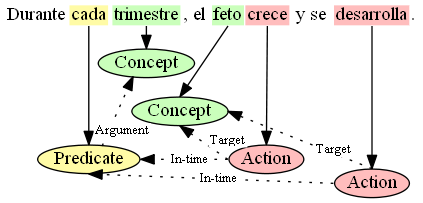
\includegraphics[width=\textwidth]{graphics/annotation_example_in_time.png}
		\caption{Ejemplo de anotación de tiempo.}
		\vspace{0.2in}
		\label{fig:annotation_example_in_time}
	\end{subfigure}
	\begin{subfigure}{3.3in}
		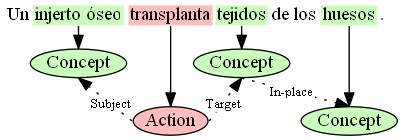
\includegraphics[width=\linewidth]{graphics/annotation_example_in_place.png}
		\caption{Ejemplo de anotación de lugar.}
		\vspace{0.2in}
		\label{fig:annotation_example_in_place}
	\end{subfigure}
	\begin{subfigure}{3.2in}
		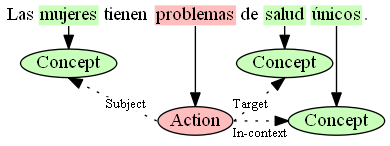
\includegraphics[width=\linewidth]{graphics/annotation_example_in_context.png}
		\caption{Ejemplo de anotación de contexto.}
		\label{fig:annotation_example_in_context}
	\end{subfigure}
	\caption{Anotación de contextualización}
\end{figure}


\begin{figure}[H]
	\centering
	\begin{subfigure}{2.4in}
		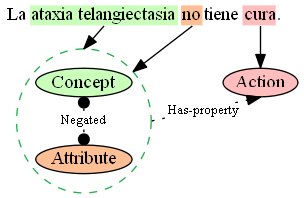
\includegraphics[width=\textwidth]{graphics/annotation_example_attribute_negated.png}
		\caption{Ejemplo de anotación del atributo negación.}
		\vspace{0.3in}
		\label{fig:annotation_example_attribute_negated}
	\end{subfigure}
	\quad
	\begin{subfigure}{2.2in}
		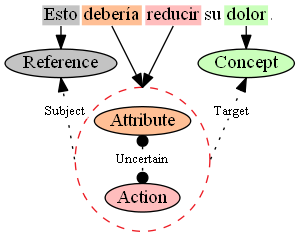
\includegraphics[width=\linewidth]{graphics/annotation_example_attribute_uncertain.png}
		\caption{Ejemplo de anotación del atributo incertidumbre.}
		\vspace{0.3in}
		\label{fig:annotation_example_attribute_uncertain}
	\end{subfigure}
	\begin{subfigure}{4.2in}
		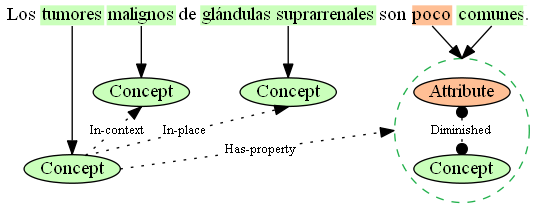
\includegraphics[width=\linewidth]{graphics/annotation_example_attribute_diminished.png}
		\caption{Ejemplo de anotación del atributo disminución.}
		\vspace{0.3in}
		\label{fig:annotation_example_attribute_diminished}
	\end{subfigure}
	\begin{subfigure}{2.3in}
		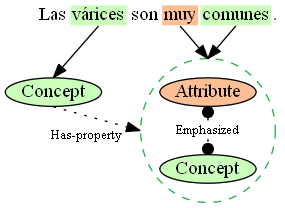
\includegraphics[width=\linewidth]{graphics/annotation_example_attribute_emphasized.png}
		\caption{Ejemplo de anotación del atributo énfasis.}
		\label{fig:annotation_example_attribute_emphasized}
	\end{subfigure}
	\caption{Anotación de los atributos}
	\label{fig:annotation_examples_attributes}
\end{figure}

\subsection{Atributos}\label{section:attributes}
Cuatro atributos booleanos\footnote{El tipo de dato lógico o booleano es en computación aquel que puede representar valores de lógica binaria, estos son dos valores, los cuales normalmente se representan como falso y verdadero. Se utiliza generalmente en la programación, estadísticas, electrónica y matemáticas mediante la utilización del álgebra booleana.} adicionales pueden ser asociados a cualquier concepto para calificarlo o describirlo un poco más. Ellos son: \textit{negated}, \textit{uncertain}, \textit{diminished} y \textit{emphasized} (en español \textit{negación}, \textit{incertidumbre}, \textit{disminución} y \textit{énfasis} respectivamente). Estos atributos son usados para evitar anotar palabras del idioma que son usadas con bastante frecuencia como \textit{no}, \textit{puede}, \textit{poco}, \textit{mucho}, y en su lugar asociar directamente el calificador correspondiente al concepto en sí. Además, los atributos capturan la negación, incertidumbre, disminución o énfasis que se pretendía en la oración, aun cuando sea implícito y no indicado explícitamente por otra palabra de la misma. Estos atributos acompañan al concepto que modifican en todas las relaciones en que este participe. En la figura \ref{fig:annotation_examples_attributes} puede verse un ejemplo anotado de cada uno de estos cuatro atributos.

\section{Formato de anotación}
\label{section:annotation_file_format}
Las anotaciones creadas con este formato son guardadas en archivos separados del documento de texto. Este último nunca es modificado. Para cada documento que vaya a ser anotado, se crea su respectivo archivo de anotación. Ambos archivos son asociados a través de su nombre, los cuales coinciden completamente exceptuando en su extensión. Las extensiones correspondientes al documento de texto y al anotado son \texttt{.txt} y \texttt{.ann} respectivamente.

En el documento anotado, las anotaciones individuales se conectan a fragmentos de texto a través de rangos de posiciones de los caracteres. Por ejemplo, si el documento comenzara así:

\begin{center}
	\doublequote{\textit{El consumo de alcohol puede causar problemas en el hogar} \dots}
\end{center}

La palabra \guillemot{\texttt{consumo}} se identifica por el rango de posiciones $3\dots10$. Las posiciones comienzan en $0$ con el inicio del documento, además, todo carácter cuenta como posición válida, incluyendo los espacios en blanco y los cambios de línea.

De manera formal, lo anterior queda expresado como: sea $\sum$ un alfabeto de símbolos, el documento $D=c_1c_2\dots c_n$ y la palabra o frase $w$ perteneciente a este, port tanto, $\exists v$ tal que $vw$ es un prefijo de $D$, entonces el rango de posiciones de $w$ en el archivo anotado comienza en $\abs{v}$ y acaba en $\abs{v}+\abs{w}$.

\subsection{Archivo de texto}
El archivo de texto debe tener como extensión \guillemot{\texttt{.txt}} y contener la información del documento original. Además, debe estar guardado en texto plano y codificado usando UTF-8\footnote{\label{note:utf8}Siglas de \textit{\textbf{U}nicode \textbf{T}ransformation \textbf{F}ormat - 8}, un formato de codificación de caracteres.}. Puede contener cambios de línea, los cuales cuentan como un símbolo.

\subsection{Archivo de anotación}
El archivo de anotación debe tener como extensión \guillemot{\texttt{.ann}}. Además, estar guardado en texto plano y codificado usando UTF-8\textsuperscript{\ref{note:utf8}}. Los tipos de anotación específicas que pueden estar presentes en este archivo se explican en las proximas secciones.

\subsection{Estructura general de la anotación}
Todas las anotaciones tienen la misma estructura básica: cada línea tiene una sola anotación específica y esta tiene un identificador único que se encuentra al comienzo de la misma. Luego, separado por un carácter TAB, se encuentra el resto de la información en la anotación específica.

El resto de la estructura de cada anotación específica varía en dependencia de los distintos tipos que hay. Esto se explica detalladamente en las siguientes secciones.

\begin{annexample}
	[backgroundcolor=cyan!13]
	{2.8in}
	{fig:general_annotation_structure}
	{Ejemplo de escritura del identificador de anotaciones}
	{Ejemplo de escritura del identificador de anotaciones.}
	T9\space\space Concept 658 664\space cuerpo\\
	R13\space in-place Arg1:T3 Arg2:T13\\
	A1\space\space Negated T10\\
	\textasteriskcentered\space\space\space same-as T1 T2
\end{annexample}

\subsection{Convenio de anotación de identificadores}
\label{subsection:id_annotation_conventions}
Todos los identificadores de anotaciones consisten en un único carácter en mayúsculas identificando el tipo de anotación y a continuación su número. Este carácter inicial es:

\vspace{-0.1in}
\begin{center}
	\begin{itemize}
		\item[•] \texttt{T}: texto
		\vspace{-0.1in}
		\item[•] \texttt{R}: relación
		\vspace{-0.1in}
		\item[•] \texttt{A}: atributo
		\vspace{-0.1in}
		\item[•] \texttt{\#}: nota o comentario
	\end{itemize}
\end{center}

\vspace{-0.1in}
Adicionalmente, un asterisco (\doublequote{\,*\,}) puede ser usado como un identificador, pero solo en casos especiales.

\subsection{Anotación de texto}
La anotación de texto es una categoría importante, incluso pudiera decirse que es la base de la anotación, pues es quien delimita los fragmentos de texto específicos que serán usados y además, sobre estos es que las relaciones y atributos surten efecto. Estas se basan en la siguiente estructura:

\begin{annexample}
	[backgroundcolor=green!13]
	{3.7in}
	{fig:text_bound_annotation_structure}
	{Estructura de anotación de texto}
	{Estructura de anotación de texto.}
	T<id>[TAB]<type>[SPACE]<span>[TAB]<text>
\end{annexample}

\begin{itemize}
	\item[•] \texttt{[TAB]} y \texttt{[SPACE]} son el carácter TAB y el carácter espacio respectivamente.
	\item[•] \texttt{<id>} es el número correspondiente a esa anotación específica.
	\item[•] \texttt{<type>} es el tipo de rol, el cual puede ser solo uno de los cuatro siguientes: {\it Concept}, {\it Action}, {\it Reference} o {\it Predicate}.
	\item[•] \texttt{<span>} son los rangos de posiciones de las palabras pertenecientes al texto que será anotado. Si este fragmento contiene más de una palabra, entonces se unirán sus rangos de posiciones usando el carácter punto y coma (\doublequote{\texttt{;}}) como separador y estas serán escsritas separadas por un carácter espacio.
	\item[•] \texttt{<text>} es el texto específico que será anotado.
\end{itemize}

Para este ejemplo, y los restantes en esta sección pertenecientes a explicar el formato de anotación, se usará el siguiente documento de ejemplo, el cual contiene una única oración:
\begin{center}
	\guillemot{\textit{Las mujeres embarazadas también pueden desarrollar diabetes, llamada diabetes gestacional.}}
	\label{sentence:annotation_example}
\end{center}

En la figura \ref{fig:text_bound_annotation_example} se puede ver el resultado de anotar el texto relevante en \hyperref[sentence:annotation_example]{el documento de prueba}.

\begin{annexample}
	[backgroundcolor=cyan!13]
	{4.1in}
	{fig:text_bound_annotation_example}
	{Ejemplo de anotación de texto}
	{Ejemplo de anotación de texto.}
	T1\space\space Concept 4 11\space\space\space\space mujeres\\
	T2\space\space Concept 12 23\space\space\space embarazadas\\
	T3\space\space Action 39 50\space\space\space\space desarrollar\\
	T4\space\space Concept 51 59\space\space\space diabetes\\
	T5\space\space Concept 69 77;78 89 diabetes gestacional
\end{annexample}

\vspace{-0.3in}
\subsection{Anotación de relaciones}
\label{section:relation_annotation}
Todas las relaciones anotadas son binarias\footnote{Una relación binaria $R$ es el subconjunto de los elementos del producto cartesiano $A_1\times A_2$ que cumplen una determinada condición: $R = \{(a_1,~a_2) : (a_1,~a_2)\in A_1\times A_2\wedge R(a_1,~a_2) = Verdadero \}$.}. Estas anotaciones siguen la siguiente estructura:

\begin{annexample}
	[backgroundcolor=green!13]
	{4.75in}
	{fig:relation_annotation_structure}
	{Estructura de anotación de texto}
	{Estructura de anotación de texto.}
	R<id>[TAB]<type>[SPACE]Arg1:T<id1>[SPACE]Arg2:T<id2>
\end{annexample}

\vspace{-0.3in}
\begin{itemize}
	\item[•] \texttt{[TAB]} y \texttt{[SPACE]} son el carácter TAB y el carácter espacio respectivamente.
	\item[•] \texttt{<id>} es el número correspondiente a esa anotación específica.
	\item[•] \texttt{<type>} es el tipo de relación anotada, el cual puede ser solo uno de los trece vistos anteriormente: {\it subject}, {\it target}, {\it domain}, {\it argument}, {\it is-a}, {\it part-of}, {\it same-as}, {\it has-property}, {\it causes}, {\it entails}, {\it in-time}, {\it in-place} o {\it in-context}.
	\item[•] \texttt{<id1>} e \texttt{<id2>} son los identificadores de las anotaciones de texto que participan en esta relación.
\end{itemize}

Es necesario tener en cuenta que este tipo de anotaciones se interpretan de izquierda a derecha, es decir, se interpretan \guillemot{\texttt{T<id1>} \textit{<type>} \texttt{T<id2>}}. Por tanto, el orden en que son anotados sus argumentos tiene vital importancia.

En la figura \ref{fig:relation_annotation_example} se puede ver el resultado de anotar las relaciones en \hyperref[sentence:annotation_example]{el documento de prueba}.

\begin{annexample}
	[backgroundcolor=cyan!13]
	{3in}
	{fig:relation_annotation_example}
	{Ejemplo de anotación de relaciones}
	{Ejemplo de anotación de relaciones.}
	R1\space\space in-context Arg1:T1 Arg2:T2\\
	R2\space\space subject Arg1:T3 Arg2:T1\\
	R3\space\space target Arg1:T3 Arg2:T4\\
	R4\space\space same-as Arg1:T3 Arg2:T5
\end{annexample}

Como se comentó anteriormente, en algunos casos especiales un asterisco (\doublequote{\,*\,}) puede ser usado en vez de un identificador. Este es el caso de la relación \texttt{same-as}, la cual es simétrica y transitiva. Ellas pueden pueden tener un asterisco al comienzo o un identificador estándar como las restantes relaciones. Cuando se utiliza un asterisco, no es necesario anotar los argumentos explícitamente junto a los identificadores, ni tampoco que sean solo dos argumentos. Por este motivo puede ser compactada y los identificadores que actúan en esta relación deben ser anotados separados por un único carácter espacio, sin importar si estos son dos o más.

A continuación en la figura \ref{fig:same_as_relation_annotation_example} se puede ver un ejemplo de anotación de este tipo en \hyperref[sentence:annotation_example]{el documento de prueba}.

\begin{annexample}
	[backgroundcolor=cyan!13]
	{1.8in}
	{fig:same_as_relation_annotation_example}
	{Ejemplo de anotación de la relación \texttt{same-as}}
	{Ejemplo de anotación de la relación \texttt{same-as}.}
	\textasteriskcentered\space\space\space same-as T3 T5
\end{annexample}

\subsection{Anotación de atributos}
Los atributos booleanos anteriormente mencionados, son asociados a su respectivo concepto a través de una relación binaria. La misma contiene un único concepto específico unido a un tipo de atributo. Cabe aclarar que, como se comentó en la sección \ref{section:attributes}, estos sintetizan una familia de palabras y por ende, semánticamente no tienen un palabra explícitamente asociada.

Las anotaciones de atributos siguen la siguiente estructura:

\begin{annexample}
	[backgroundcolor=green!13]
	{2.87in}
	{fig:attribute_annotation_structure}
	{Estructura de anotación de texto}
	{Estructura de anotación de texto.}
	A<id>[TAB]<type>[SPACE]T<id1>
\end{annexample}

\vspace{-0.2in}
\begin{itemize}
	\item[•] \texttt{[TAB]} y \texttt{[SPACE]} son el carácter TAB y el carácter espacio respectivamente.
	\item[•] \texttt{<id>} es el número correspondiente a esa anotación específica.
	\item[•] \texttt{<type>} es el tipo de atributo anotado, el cual puede ser solo uno de los cuatro vistos anteriormente: {\it Negated}, {\it Uncertain}, {\it Diminished} o {\it Emphasized}.
	\item[•] \texttt{<id1>} es el identificador de la anotación de texto que es modificada por este atributo.
\end{itemize}

En la figura \ref{fig:attribute_annotation_example} se puede ver el resultado de anotar el único atributo contenido en \hyperref[sentence:annotation_example]{el documento de prueba}.

\begin{annexample}
	[backgroundcolor=cyan!13]
	{1.7in}
	{fig:attribute_annotation_example}
	{Ejemplo de anotación de atributo}
	{Ejemplo de anotación de atributo.}
	A1\space\space Uncertain T3
\end{annexample}

\subsection{Anotación de comentarios}
Un comentario es texto que no se procesa, por lo que sirve para escribir notas a modo de guía. Las anotaciones de comentarios siguen la siguiente estructura:

\begin{annexample}
	[backgroundcolor=green!13]
	{2.1in}
	{fig:comment_annotation_structure}
	{Estructura de anotación de comentarios}
	{Estructura de anotación de comentarios.}
	\#<id>[SPACE]<comment>
\end{annexample}

\vspace{-0.2in}
\begin{itemize}
	\item[•] \texttt{[SPACE]} es el carácter espacio.
	\item[•] \texttt{<id>} es el número correspondiente a esa anotación específica. Este no es obligatorio para anotar comentarios.
	\item[•] \texttt{<comment>} es el comentario en sí, y puede contener cualquier texto.
\end{itemize}

En la figura \ref{fig:comment_annotation_example} se puede ver un ejemplo de un comentario anotado.

\begin{annexample}
	[backgroundcolor=cyan!13]
	{4.8in}
	{fig:comment_annotation_example}
	{Ejemplo de anotación de comentario}
	{Ejemplo de anotación de comentario.}
	\# Las mujeres embarazadas también pueden desarrollar\\
	\# diabetes, llamada diabetes gestacional.
\end{annexample}

\subsection{Consideraciones finales}\label{section:annotation_conventions}
Las oraciones anotadas en el documento con extensión \guillemot{\texttt{.ann}} deben estar en el mismo orden con el que aparecen en el documento de texto con extensión \guillemot{\texttt{.txt}}. Además, no es necesario que todas las oraciones en el documento de texto sean anotadas, incluso puede que ninguna lo esté.

Como se vio en la sección \ref{subsection:id_annotation_conventions}, la letra inicial del identificador debe ser mayúscula, no obstante, no importa si es minúscula, aunque siempre guiarse por los convenios es una buena práctica.

Por otra parte, el convenio de anotación de los tipos es hacerlo con la primera letra en mayúscula y el resto en minúsculas para los textos y atributos, mientras que para las relaciones se debe anotar completamente en minúsculas.

Además, el orden de las anotaciones en el archivo no es relevante y tampoco lo son los números específicos de los identificadores. Aunque por cuestión de estética y para una mejor comprensión del anotador, se recomienda escribir siempre las anotaciones de texto primero, luego las relaciones y por último los atributos. En caso de los identificadores, estos deberían comenzar con el número $1$ y continuar la secuencia de forma incremental de uno en uno.

Por último, es recomendable ordenar las anotaciones de texto respecto a la posición inicial de la primera palabra en estos. Las relaciones deben estar ordenadas por los identificadores de sus argumentos, es decir, ordenar primero por el identificador del primer argumento y en caso de que varios coincidan, ordenar por el del segundo argumento.

Como caso especial están las anotaciones de relaciones de igualdad que comienzan con asteriscos, las cuales deben ser ordenadas entre ellas con igual criterio que las demás relaciones, pero deben ir después de estas. Estas anotaciones deberían comenzar siempre con un asterisco, aunque, como se mencionó en la sección \ref{section:relation_annotation}, no tiene ningún inconveniente hacerlo de manera similar a las demás.

Por último, los atributos deben ordenarse de manera similar, pero en este caso, guiándose por el identificador su único argumento.

Siguiendo las recomendaciones anteriores, \hyperref[sentence:annotation_example]{el documento de prueba} quedaría anotado de la siguiente manera:

\begin{annexample}
	[backgroundcolor=cyan!13]
	{4.8in}
	{fig:annotated_document_example}
	{Ejemplo de anotación de comentario}
	{Ejemplo de anotación de comentario.}
	\# Las mujeres embarazadas también pueden desarrollar\\
	\# diabetes, llamada diabetes gestacional.\\
	T1\space\space Concept 4 11\space\space\space\space mujeres\\
	T2\space\space Concept 12 23\space\space\space embarazadas\\
	T3\space\space Action 39 50\space\space\space\space desarrollar\\
	T4\space\space Concept 51 59\space\space\space diabetes\\
	T5\space\space Concept 69 77;78 89 diabetes gestacional\\
	R1\space\space in-context Arg1:T1 Arg2:T2\\
	R2\space\space subject Arg1:T3 Arg2:T1\\
	R3\space\space target Arg1:T3 Arg2:T4\\
	\textasteriskcentered\space\space\space same-as T3 T5\\
	A1\space\space Uncertain T3
\end{annexample}

\section{Anotación automática de documentos}
El proceso de anotación de un documento, llevado a cabo por un humano, puede ser engorroso. Dado que un corpus contiene varios de estos, anotarlo puede tomar gran cantidad de tiempo.

No es de extrañar que con el avance tecnológico y científico, principalmente de la inteligencia artificial en este último, este proceso pueda automatizarse. Los avances en este aspecto tienen ventajes y desventajas, a la vez de márgenes de errores y precisión.

En la competencia \textit{eHealth-KD Challenge} presentada en \textit{IberLEF 2019}~\cite{ref:17} e \textit{IberLEF 2020}~\cite{ref:18} tomaron lugar sistemas automáticos para la anotación de corpus~\cite{ref:21}. Las propuestas que compitieron están entrenadas para hacerlo en textos médicos del idioma español y usando el modelo de anotación explicado en esta investigación~\cite{ref:21,ref:19}. De igual forma, otros pueden ser encontrados en la literatura para anotar automáticamente documentos pertenecientes a diferentes dominios e idiomas.

\section{Análisis del corpus}
El corpus usado~\cite{ref:20} fue construido a partir de un fichero \textit{XML}\footnote{Siglas en inglés de \textit{e\textbf{X}tensible \textbf{M}arkup \textbf{L}anguage}, un lenguaje de marcado desarrollado por el \textit{World Wide Web Consortium} (W3C).} tomado del sitio web de \textit{Medline} el $9$ de enero de $2018$, específicamente a las $02:30:31$. \textit{Medline} fue producida y es mantenida por la Biblioteca Nacional de Medicina de los Estados Unidos. Recoge referencias bibliográficas de los artículos publicados en aproximadamente $5,500$ revistas médicas desde $1966$. Actualmente reúne más de $30,000,000$ de citas. Cada registro de \textit{Medline} es la referencia bibliográfica de un artículo científico publicado en una revista médica, con los datos bibliográficos básicos de un artículo: título, autores, nombre de la revista, año de publicación, entre otros. Esto permite la recuperación de estas referencias posteriormente en una biblioteca o a través de un \textit{software} específico de recuperación.

\begin{figure}[H]
	\begin{center}
		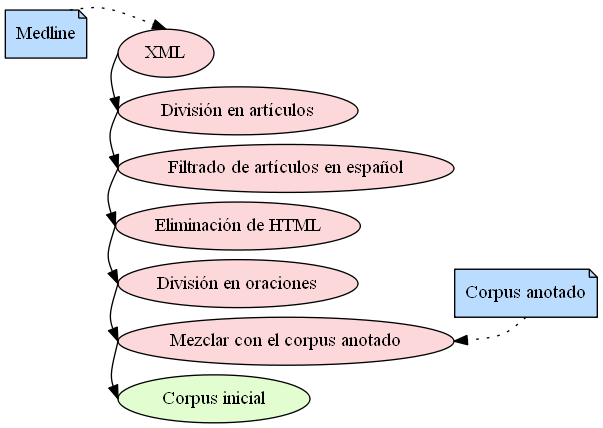
\includegraphics[height=3.4in]{graphics/corpus_processing.png}
		\caption[Esquema del procesamiento inicial del corpus]{Esquema del procesamiento inicial del corpus.}
		\label{fig:corpus_processing}
	\end{center}
\end{figure}

\vspace{-0.2in}
En la figura \ref{fig:corpus_processing} puede verse una representación esquemática del procesamiento inicial que se le hace al corpus de \textit{Medline}, el cual de forma análoga puede aplicarse a otros.